%----------------------------------------------------------------------
% Harnessing cloud computing for high capacity analysis of neuroimaging
% data from NDAR
%
% Poster for OHBM 2015
%
% Contributing authors: Daniel Clark, Cameron Craddock
%----------------------------------------------------------------------

%----------------------------------------------------------------------
% Document class, packages, and formatting
%----------------------------------------------------------------------
\documentclass[final,hyperref={pdfpagelabels=false}]{beamer}

%% Packages
\usepackage{grffile}
\usepackage[english]{babel}
\usepackage[latin1]{inputenc}
\usepackage{amsmath,amsthm, amssymb, latexsym}
%\usepackage[framemethod=tikz]{mdframed}
%\usepackage{times}\usefonttheme{professionalfonts}  % obsolete
%\usefonttheme[onlymath]{serif}
%\boldmath
\usepackage{enumerate}
%\usepackage[orientation=portrait,size=custom,width=83.96,height=101,scale=1]{beamerposter}
\usepackage[orientation=portrait,size=custom,width=96,height=70,scale=1]{beamerposter}
%\usepackage[orientation=portrait,width=89,height=102,scale=1.1,debug]{beamerposter}
%\usepackage[orientation=portrait,size=a0,scale=1.4,debug]{beamerposter}
% change list indention level
% \setdefaultleftmargin{3em}{}{}{}{}{}
%\usepackage{snapshot} % will write a .dep file with all dependencies, allows for easy bundling

\usepackage{array,booktabs,tabularx}

%% Formatting
\mode<presentation>{\usetheme{CMINKI}}
\newcolumntype{Z}{>{\centering\arraybackslash}X} % centered tabularx columns
\newcommand{\pphantom}{\textcolor{ta3aluminium}} % phantom introduces a vertical space in p formatted table columns??!!
% Column sizing
\newlength{\columnheight}
\setlength{\columnheight}{72cm}

%\graphicspath{{figures/}}
\listfiles

%----------------------------------------------------------------------
% Title Block
%----------------------------------------------------------------------
%% Title
\title{\vskip1ex\Huge Harnessing cloud computing for high capacity analysis of neuroimaging data from NDAR}

%% Author
\author{\Large Daniel Clark$^1$, Christian Haselgrove$^2$, David Kennedy$^2$, Zhizhong Liu$^3$,\\[.5ex]Michael Milham$^1$, Petros Petrosyan$^4$, Carinna Torgerson$^3$, John Van Horn$^3$, Cameron Craddock$^1$}
\institute[NKI]{$^1$Child Mind Institute, New York, NY, $^2$ University of Massachuttes Medical School, Worcester, MA, $^3$University of Southern California, Los Angeles, CA, $^4$UCLA, Los Angeles, CA, $^5$Nathan S. Kline Institute for Psychiatric Research, Orangeburg, NY}

%% Poster info
\posternum{\Large 3535 Thursday 12:45}
\date[June 18th, 2015]{June 18th, 2015}

%----------------------------------------------------------------------
% Poster content
%----------------------------------------------------------------------
\begin{document}
\begin{frame}
    \begin{columns}
    % ---------------------------------------------------------%
    % Set up a column 
    \begin{column}{.5\textwidth}
      %\begin{beamercolorbox}[center,wd=\textwidth]{postercolumn}
        %\begin{minipage}[T]{.98\textwidth}  % tweaks the width, makes a new \textwidth
          \parbox[t][\columnheight]{\textwidth}{ % must be some better way to set the the height, width and textwidth simultaneously
            % Since all columns are the same length, it is all nice and tidy.  You have to get the height empirically
            %----------------------------------------------------------------------
            % Introduction
            %----------------------------------------------------------------------
            \begin{block}{Introduction}
              \begin{itemize}
                  \item The National Database for Autism Research (NDAR) hosts a vast collection of neuroimaging datasets that can be processed and utilized to yield significant scientific discoveries.
                  \item This amount of resources necessitates a high-performance computing (HPC) infrastructure, which is not always readily available for researchers in-house.
                  \item Amazon Web Services (AWS) Elastic Compute Cloud (EC2) computing service offers a ``pay as you go" model that allows researchers to utilize HPC performance without the up-front captial costs and maintenance of an in-house solution.
                  \item The developers of the Laboratory of Neuro Imaging (LONI) Pipeline, the Neuroimaging Informatics Tools and Resources Clearinghouse (NITRC) Computational Environment (CE) and the Configurable Pipeline for the Analysis of Connectomes (C-PAC) have implemented pipelines in EC2 that interface with NDAR
              \end{itemize}
            \vfill
            \end{block}
            %----------------------------------------------------------------------
            % Methods
            %----------------------------------------------------------------------
            \begin{block}{Methods}
                \begin{column}{.5\textwidth}
                    {\bf LONI Pipeline} 
                    \begin{itemize}
					    \item The LONI Pipeline software was extended to include new pipeline modules to access data from the NDAR database, transfer input data out of Amazon S3 (Simple Storage Service), and to load results back into S3$^{1}$
						\item A pipeline was constructed to extract cortical thickness and subcortical region volume data from structural MRI images in the NDAR database, which included:
						\begin{enumerate}
							\item Reorient images to standard orientation using FSL's reorient2std module
							\item Extract cortical thickness using FreeSurfer recon-all
							\item Calculate volumes of subcortical regions using FSL's BET and FIRST all
						\end{enumerate}
						\item The resulting pipeline was used to process 780 T1-weighted structural images and return the results to NDAR
                    \end{itemize}
                    \vskip1ex
                \end{column}
                %\vskip1ex
                \begin{column}{.5\textwidth}
                    \begin{figure}
                        \begin{center}
                            \includegraphics[width=.9\textwidth]{loni_pipeline.eps}
                        \end{center}
                        \caption{\label{fig:roi_metrics}Graphical layout of the constructed pipeline}
                    \end{figure}
                \end{column}
				
                {\bf Configurable Pipeline For the Analysis of Connectoms (C-PAC)} 
                \begin{itemize}
				    \item C-PAC modules were written in Python to build input data lists by querying NDAR, read input data from S3, write processed results to S3 and write values back to the NDAR database$^{2}$
					\item New pipelines were created to perform the ANTS cortical thickness$^{3}$ procedure and the Preprocessed Connectomes Project's Quality Assessment Protocol (\url{http://preprocessed-connectomes-project.github.io/quality-assessment-pipeline})$^{4}$
					\begin{enumerate}
						\item Reorient images to standard orientation using FSL's reorient2std module
						\item Extract cortical thickness using FreeSurfer recon-all
						\item Calculate volumes of subcortical regions using FSL's BET and FIRST all
					\end{enumerate}
					\item The resulting pipeline was used to process 780 T1-weighted structural images and return the results to NDAR
                \end{itemize}
                \vskip1ex
                \begin{column}{.47\textwidth}
                    \begin{itemize}
                        \item Launched an AWS-hosted miNDAR database by querying NDAR website for the data of interest (e.g. from a particular study)
                        \item Built a subject list by querying the database for subjects of interest to pass to our pipeline
                        \item Launch an AWS EC2 HPC cluster using Starcluster
                        \item Log into the cluster and submit a Sun Grid Engine job using our pipeline software and the subject list
                        \item The pipeline software will process the data, store raw outputs in an AWS S3 bucket and insert S3 filepaths and output measures into miNDAR database
                    \end{itemize}
                \end{column}
                \begin{column}{.47\textwidth}
                    \begin{figure}
                        \begin{center}
                            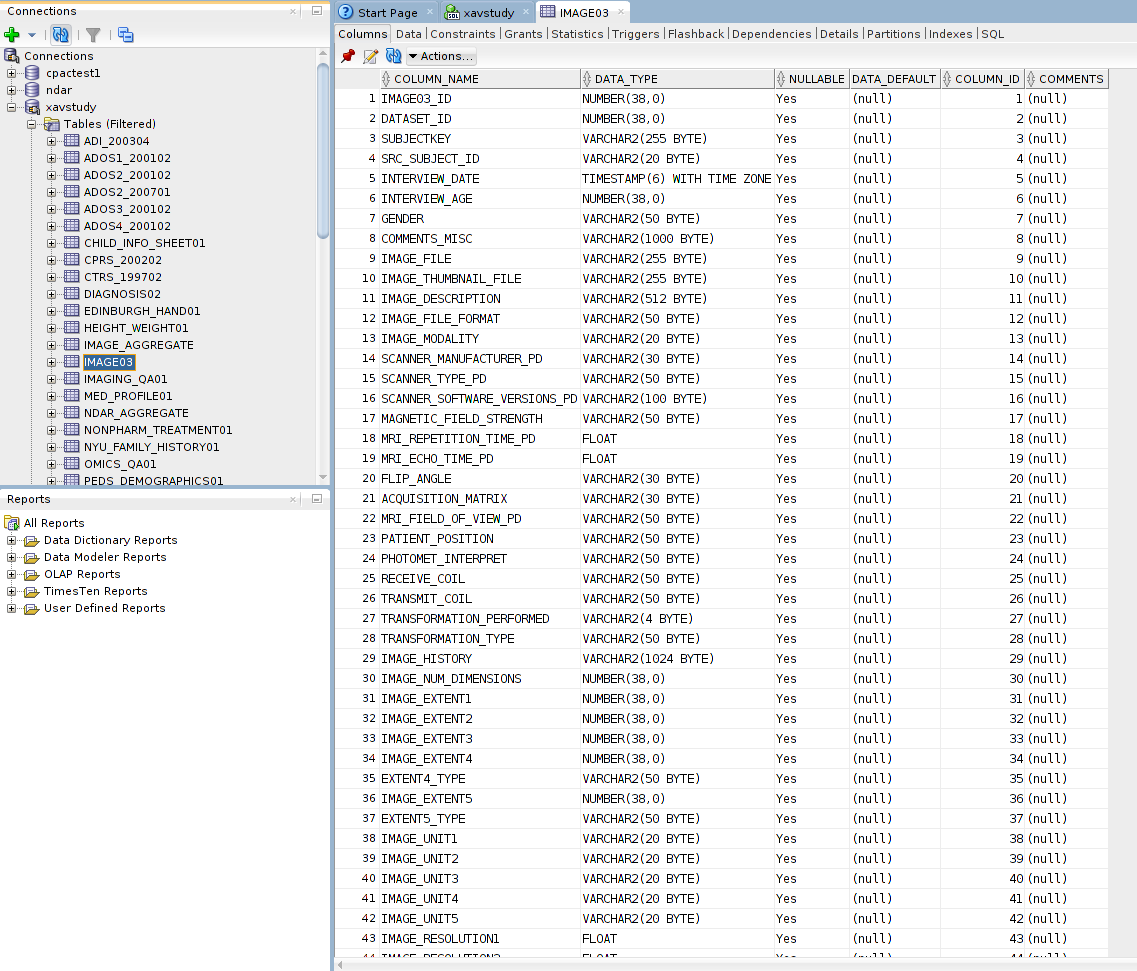
\includegraphics[width=.9\textwidth]{mindar.png}
                        \end{center}
                        \caption{\label{fig:mindar}miNDAR database}
                    \end{figure}
                \end{column}
            \begin{figure}
                \begin{center}
                    \includegraphics[width=.60\textwidth]{flow_chart.eps}
                \end{center}
                \caption{\label{fig:processingflow}Flow chart of neurofeedback experiment.}
            \end{figure}    
            \vfill              
            \end{block}
          }
        %\end{minipage}
      %\end{beamercolorbox}
    \end{column}
    % ---------------------------------------------------------%
    % end the column

    % ---------------------------------------------------------%
    % Set up a column 
    \begin{column}{.5\textwidth}
      %\begin{beamercolorbox}[center,wd=\textwidth]{postercolumn}
       % \begin{minipage}[T]{.98\textwidth} % tweaks the width, makes a new \textwidth
          \parbox[t][\columnheight]{\textwidth}{ % must be some better way to set the the height, width and textwidth simultaneously
            % Since all columns are the same length, it is all nice and tidy.  You have to get the height empirically
            % ---------------------------------------------------------%
            % fill each column with content
            \begin{block}{Results}
				\begin{center}
			
			\begin{table}
			  \caption{Processing completed as a part of the effort. Nodes corresponds to the number of hosts used in the calculation. PF is parallelization factor and corresponds to the number of jobs ran in parallel on each node. On demand instances were used for the master node and spot instances were used for all computation nodes in the cluster. CPU Time is the total amount of time required to perform the computation and Wall Time is the amount of time that passed. \# DS: Number of datasets. CPD: Cost Per Dataset. C-PAC: Configurable Pipeline for the Analysis of Connectomes. NITRC-CE: NITRC Computational Environment}
			  \begin{tabular}{lrl*{6}{r}}
				  {\bf Processing} & {\bf \# DS} & {\bf Platform} & {\bf Nodes} & {\bf PF} & {\bf CPU Time} & {\bf Wall Time} & {\bf Cost} & {\bf CPD}\\
			      \hline
				  ANTS Cortical Thickness & 3197 &  & 20 & 8 & 23,018 & 147 & \$760.24 & \$0.24\\
			 	  Resting state fMRI processing w/ 4 strategies & 1112 & C-PAC  & 20 & 3 & 834 & 22 & \$80.54 & \$0.07 \\
				  Quality Assessment Protocol & 1112 & & 20 & 4 & 380 & 14 & \$19.02 & \$0.02 \\
				  \hline
				  Freesurfer recon-all & 986 &  & 4 & 32 & 23,664 & 193 & \$211.44 & \$0.21 \\
				  FSL FIRST & 1247 & NITRC-CE & 4 & 32 & 208 & 3 & \$2.19 & $>$ \$0.01 \\
				  Temporal QA & 1349 &  & 4 & 32 & 450 & 13 & \$4.69 & $>$ \$0.01 \\
				  \hline
				  Freesurfer recon-all and FSL FIRST & 780 & LONI Pipeline & 20 & 32 & 18,720 & 49 & \$252.36 & \$0.32 \\
			 \end{tabular}
			\end{table}
			 \end{center}
              \begin{column}{.47\textwidth}

                  %\begin{figure}
                  %    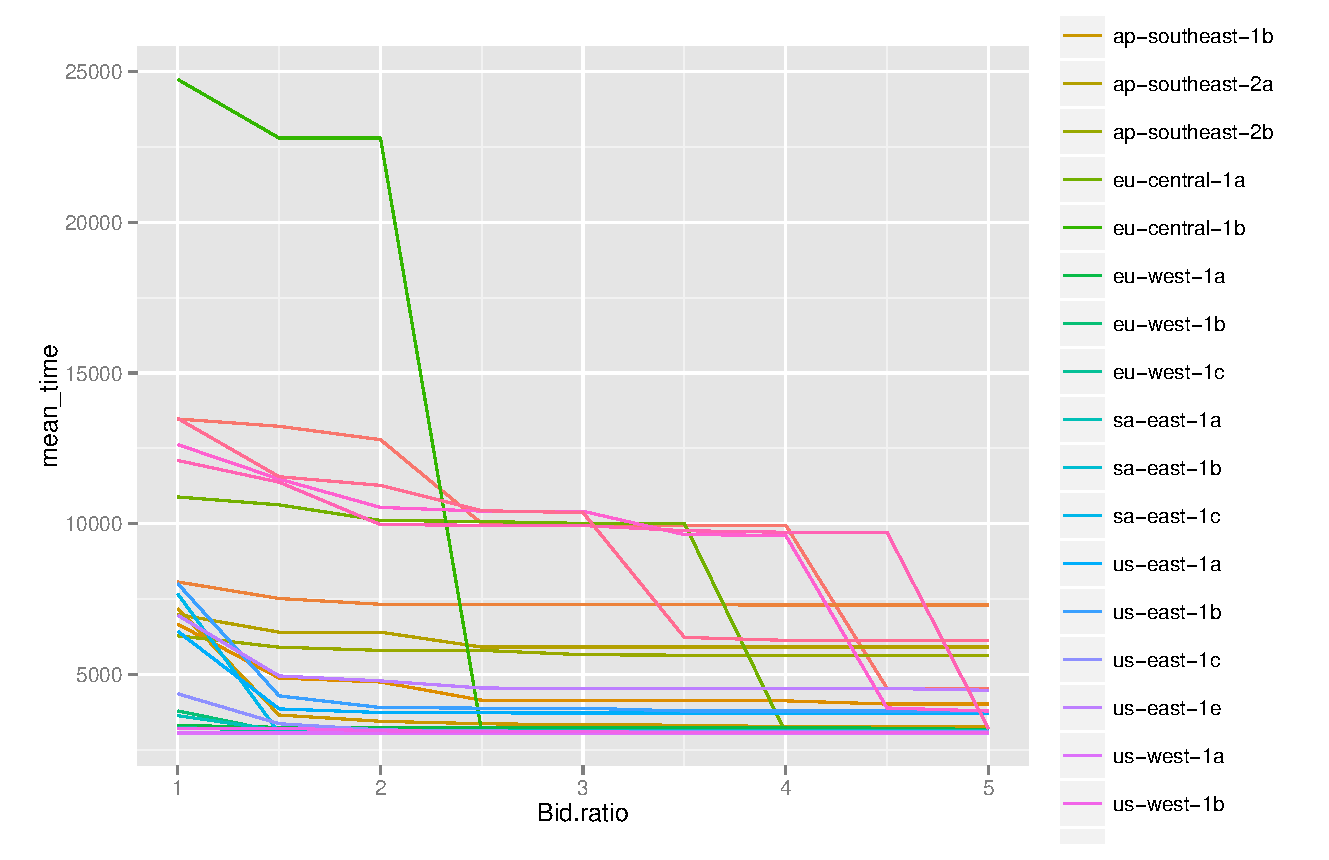
\includegraphics[width=.99\textwidth]{br_vs_time_fs.eps}
                  %    \caption{\label{fig:best_worst}Bid ratio vs Computation time in minutes for the Freesurfer pipeline}
                  %\end{figure}
                  %\vskip2ex
                  %\begin{figure}
                  %    \includegraphics[width=.99\textwidth]{inter_subject.eps}
                  %    \caption{\label{fig:inter_subject} Performance across particpants (A) differs between feedback and neurofeedback scans as determined by their order (B).}
                  %\end{figure}
                  \end{column}
                  \begin{column}{.49\textwidth}
                      \vskip4ex
                  \begin{figure}
                      \includegraphics[width=.99\textwidth]{beh_correlates.eps}
                      \caption{\label{fig:beh_correlates} Inter-individual variation in preformance correlates with behavioral measures.}
                  \end{figure}
              
                  \begin{itemize}
                       \item As shown in figure \ref{fig:best_worst} models learned for the best and worst performing participants match
                             with the canonical pattern of the default network.
                       \item The best participant was able to follow the instructures very well \ref{fig:best_worst}, the worst seems
                             to have been corrupted by noise.
                       \item Figure \ref{fig:inter_subject} shows 12 of the subjects were able to modulate the DN at above chance levels,
                             performance on feedback runs is consistent independent of order, but performance on nonfeedback runs improves
                             if they occur after feedback runs.
                       \item Measures that were significantly associated with DN regulation include ($p<0.05$, FDR corrected):  the affect intensity measure (AIM), ruminative responses scale (RRS), and the imaginal processes inventory. 
                  \end{itemize}
              \end{column}
            \end{block}
            \begin{block}{Conclusion}
              \begin{itemize}
                   \item We developed a system for measuring DN regulation using realtime neurofeedback. 
                   \item Participants were able to modulate their DN activity and their ability to do so was correlated with phenotype. 
                   \item This system provides a new experimental paradigm for understanding network dysregulation and how it maps to 
                        disease states and phenotype.
                   
                   
              \end{itemize}
            \end{block}
            \begin{block}{References and Acknowledgements}
                    1. Sonuga-Barke, E. et al. (2007), Neuroscience and Biobehavioral Reviews 31:977-986.\\
                    2. Broyd, S. J. et al. (2009), Neuroscience and Biobehavioral Reviews 33: 279-296.\\
                    3. Sheline, Y.I. et al. (2009), PNAS 106: 1942-1947.\\
                    4. Whitfield-Gabrieli, S. et al. (2009), PNAS 106: 1279-1284.\\
                    5. Hamilton, J.P. et al. (2011), Biol. Psychiatry 70: 327-333.\\
                    6. Sylvester, C.M. et al. (2012), Trends Neurosci. 35, 527-535.\\
                    7. Castellanos, F.X. et al. (2012), Trends Cogn. Sci. 16, 17-26.\\
                    8. LaConte, S.M. et al. (2004). Human Brain Mapping, 11: 2551.\\
                    9. LaConte, S.M. et al. (2011). NeuroImage, 56(2), 440-454.\\
                    10. Cox, R.W. (1996) Comput. Biomed. Res. 29: 162-173.\\
                    \vskip1ex
               Data collection and salary support was provided by a NARSAD Young Investigator Award to RCC.
             \end{block}
          }
          % ---------------------------------------------------------%
          % end the column
      %  \end{minipage}
      %\end{beamercolorbox}
    \end{column}
    % ---------------------------------------------------------%
    % end the column
  \end{columns}
\end{frame}
\end{document}


%%%%%%%%%%%%%%%%%%%%%%%%%%%%%%%%%%%%%%%%%%%%%%%%%%%%%%%%%%%%%%%%%%%%%%%%%%%%%%%%%%%%%%%%%%%%%%%%%%%%
%%% Local Variables: 
%%% mode: latex
%%% TeX-PDF-mode: t
%%% End:
